
\subsection{Recovery system}
Our recovery system was designed to slow down the descent rate of the payload to a safe and controlled speed which may vary depending on weather conditions (we will discuss it a bit later on). The payload’s recovery system ensures a safe and controlled descent to the ground via a deployed parachute after reaching maximum altitude.

\subsubsection{Parachute}

The key (the most important element) is the hemispherical parachute. 
\begin{wrapfigure}{l}{0.26\textwidth}
    \centering
    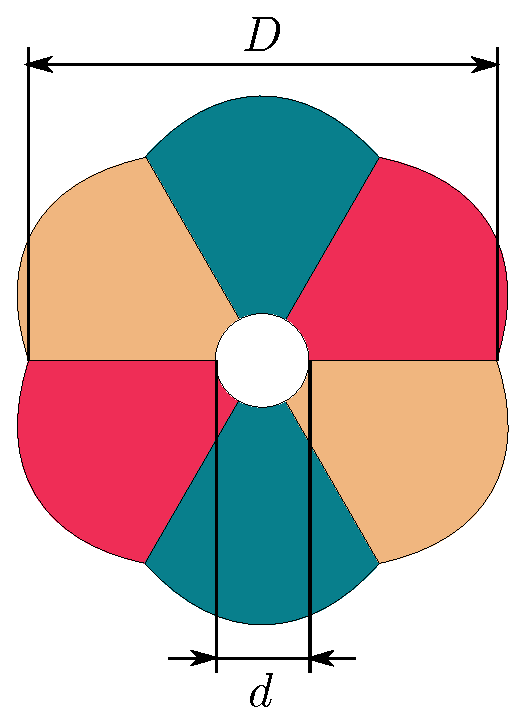
\includegraphics[width=3.75cm]{img_canopy2.eps}
    \caption{\small{Parachute design.}}
    \label{fig:software_fiagram}
\end{wrapfigure}
We have chosen this parachute type because our mission implies only a descent through the atmosphere, and we do not intend a targeted one. The parachute will be opened right after the helicopter’s payload’s launch and fixed to the can in six points to limit its rotation during descent. For the connection between the parachute and the payload, we will use six durable and lightweight ropes weighing only 1 gram/meter. The shock cord will connect the nose cone and the body tube and, depending on the kind of parachute we will use, it will be 75 or 40,5 cm long. 

Besides the parachute, we will make sure to have two secondary systems for the on-ground recovery of the payload. These systems are based on GPS coordinates provided during descent, and a loud buzzer; both are activated after landing once our sensors record no velocity. The bright colour of the can and parachute should aid the recovery team in finding the CanSat.      

To ensure the success of the recovery process, we have thought about designing the parachute system to ensure both the need for a longer flight time to conduct accurate atmospheric analysis during the descent phase in good weather conditions (1st parachute, 5 m/s), as well as the need for a fast descent in case of bad weather conditions (2nd parachute, 9 m/s). It is worth noting that the calculations we will use to determine the descent rate also take into account the time factor, which is crucial for a successful recovery.

For the values in the table we used the following formulas:
\begin{equation}\label{eq1}
S=\frac{2mg}{C_d \rho V^2}, \quad\quad D = \sqrt{\frac{4S}{\pi}}
\end{equation}

\begin{table}[htbp]
\centering
\arrayrulecolor{CDOSRPrimary}
\begin{tabular}{>{\centering\arraybackslash}lcc}
\rowcolor{CDOSRPrimary}
\hline
\textbf{\color{white!50}{Parameter}} & \multicolumn{1}{|c|}{\textbf{\color{white!50}{1st Parachute}}}  & \textbf{\color{white!50}{2nd Parachute}} \\
\hline
Surface & 0.1841 m$^{2}$ & 0.0568 m$^{2}$\\
Diameter & 0.4843 m $\approx$ 50 cm & 0.2691 m $\approx$ 27 cm \\
\hline
\end{tabular}
\caption{Surface and diameter for the parachutes}
\end{table}


To calculate the dimensions required for the parachute, we considered the following constant parameters, including physical constants and canopy parameters.

\begin{table}[htbp]
\centering
\arrayrulecolor{CDOSRPrimary}
\begin{tabular}{>{\centering\arraybackslash}lc}
\rowcolor{CDOSRPrimary}
\hline
\multicolumn{1}{|c|}{\textbf{\color{white!50}{Parameter}}}  & \textbf{\color{white!50}{Value}} \\
\hline
$g$ - gravitational acceleration & \SI{9.81 }{\meter\per\square\second} \\
\rowcolor{CDOSRSecondary!50}$\rho$ - air density & \SI{1.225}{\kilogram\per\cubic\metre} \\
$v$ - descent velocity & 5 and 9 \SI{}{\meter\per\second} \\
\rowcolor{CDOSRSecondary!50}$m$ - CanSat mass & \SI{0.30}{\kilogram} \\
$C_D$ - Drag coefficient & 0.8 \\
\rowcolor{CDOSRSecondary!50}$n$ - number of gores & 6 \\
\hline
\end{tabular}
\caption{Constant parameters and their values}
\end{table}


The hemispherical parachutes with 6 gores and an additional spill hole of diameter d = 10\% of the canopy’s diameter, D on the top, is our preferred primary recovery system due to its high drag coefficient per area, which allows for a lightweight parachute. This spill hole helps with air transition along the parachute, preventing oscillations during descent.

